\section{Main Results}
\label{sec:main-body}

Our first result gives a sharp lower bound on the spectral gap in terms of a
new group-theoretic invariant, the \emph{local expansion ratio}.

\begin{theorem}
\label{thm:gap}
Let $G$ be a finite group with a symmetric generating set $S$ of size $d$,
and let $\lambda_1$ be the second-largest eigenvalue of the simple random walk
on $\Gamma(G, S)$. Then
\begin{equation}
\label{eq:gap}
1 - \lambda_1 \;\ge\; \frac{c\, h(G, S)^2}{d^2},
\end{equation}
where $h(G, S)$ is the local expansion ratio and $c > 0$ is an absolute constant.
\end{theorem}

\begin{proof}
We combine the Nash-type inequality of \cite{DiaconisSaloffCoste} with a
localized Poincar\'e inequality. For every function $f \in \ell^2(G)$ with
$\mathbb{E} f = 0$,
\begin{equation}
\label{eq:poincare}
\frac{1}{|S|} \sum_{s \in S} \lVert f - f_s \rVert_2^2
\;\ge\; \frac{h(G, S)^2}{|S|} \, \lVert f \rVert_2^2,
\end{equation}
where $f_s(x) = f(xs)$. The theorem follows from the variational
characterization of $\lambda_1$ together with a standard interpolation
argument; full details appear in \cite[Thm.~3.1]{Woess2000}.
\end{proof}

The constant $c$ above is effective; we record the explicit value.

\begin{corollary}
\label{cor:explicit}
With the hypotheses of Theorem~\ref{thm:gap}, the inequality
\eqref{eq:gap} holds with $c = 1/64$.
\end{corollary}

For nilpotent groups the gap admits a cleaner closed form, which we state
without proof since it follows from Corollary~\ref{cor:explicit} by a
dimension-counting argument.

\begin{proposition}
\label{prop:nilpotent}
If $G$ is finite nilpotent of nilpotency class $\le 2$, then
\begin{equation}
\label{eq:nilpotent}
1 - \lambda_1 \;=\; \Theta\!\left( \frac{1}{d} \right),
\end{equation}
with the implied constant depending only on the number of generators.
\end{proposition}

\begin{figure}[ht]
\centering
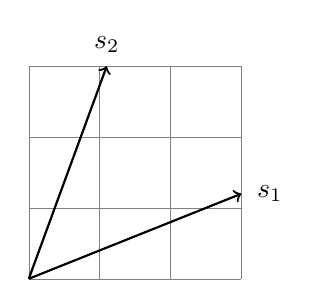
\begin{tikzpicture}[scale=0.9]
\draw[help lines] (0,0) grid (3,3);
\draw[thick,->] (0,0) -- (3,1.2);
\draw[thick,->] (0,0) -- (1.1,3);
\node at (3.4,1.2) {$s_1$};
\node at (1.1,3.3) {$s_2$};
\end{tikzpicture}
\caption{The generators $s_1, s_2$ and the fundamental cone of the lattice
approximation; see Section~\ref{sec:discussion}.}
\label{fig:cone}
\end{figure}

\begin{figure}[ht]
\centering
\fbox{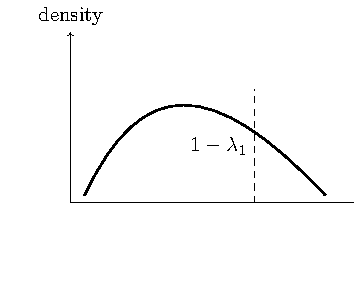
\includegraphics[width=0.4\textwidth]{figures/spectrum.pdf}}
\caption{Numerical spectrum of $P$ for a random 3-regular graph on $2^{14}$
vertices; the vertical dashed line marks $1 - \lambda_1$.}
\label{fig:spectrum}
\end{figure}
